\chapter{Categoriality and continuity in the sounds of language}
\label{chapter_pandp}

A central topic of debate in recent years has concentrated on the question of how phonology, with its categorical representations, and phonetics, with its continuous signals, relate to each other. Although concerned with the same object of study -- the sounds of speech and how they are used in communication -- phonetics and phonology share a long tradition of separation. 

This separation of the two fields at least partly originated from the fact that speech is indeed found to be concrete and continuous, yet at the same time abstract and categorical. Humans produce the acoustic signals we consider as speech sounds by moving their articulators. Both motion and acoustic output can be characterised as continuous. But the sounds of speech have been ascribed an abstract, symbolic nature in the function they serve as part of language \citep{Ladd2014,Pierrehumbert1990}. This dual nature of speech sounds is at the root of the observation that it is possible for ``two physical (acoustic) events that are objectively quite different to count as instances of the same category in the symbolic system, and for two physical events that are objectively very similar to count as instances of two different categories" \citep[29]{Ladd2014}. Many researchers have acknowledged throughout the history of linguistics that the search for an adequate characterisation of speech is not achieved with the mere description of the physical aspects of the sounds of language but has to include the mental or cognitive representations of sounds. Likewise, the description in terms of a purely abstract system void of reference to the phonetic substance proves unpromising as well, since ``phonological units and processes are what they are largely due to the physical and physiological structure of the speech mechanism" \citep[155]{Ohala1990}.

This chapter is concerned with how phonetics, phonology and their relation have been characterised by taking a brief look at some history of the fields and discussing several problems arising through a strict separation of categorical, symbolic from continuous, physical aspects that has been assumed by many models. The chapter also concentrates on which solutions have been provided more recently in the literature.

\section{Phonetics and phonology}

The physical, continuous nature of speech is traditionally treated as the domain of \emph{phonetics}. The cognitive, categorical nature of speech is attributed to the field of \emph{phonology}. While scholars working on various aspects of speech sounds did not assume a strong division between the two domains for a long time, the 20th century brought a ``split between phonetics and phonology" \citep[680]{Ohala1997}. Ferdinand de Saussure's work, in introducing the distinction between \emph{parole} and \emph{langue}, played an important role in laying the foundations of the division between phonetics and phonology. This division was spelled out more clearly by \cite{Trubetzkoy1958} -- although \cite{DurandLaks2002} note that Saussure's use of the terms ``phonetics" and ``phonology" was slightly different from Trubetzkoy's. \citet[7]{Trubetzkoy1958} proposed a division between two disciplines (``Lautlehren") each with its own name, object of study and methodology. While phonetics in his view is concerned with the physical form of speech and consequently has to use the methods of the natural sciences, phonology is concerned with the meaning of speech sounds in language, their symbolic character and has to use the methods of the humanities and social sciences. In Saussurean terms, the former discipline studies the sound pattern of parole while the latter studies the sound pattern of langue \citep{Culler1986,Ladd2014}. This division had great impact on the development of linguistics, the fields of phonetics and phonology and on the way scholars have since viewed language and speech in general. While the division seems natural to many and is commonly taught in introductory courses in linguistics, it has also been the subject of one of the most important debates in the study of language in recent years.

One of the major building blocks for a clear-cut separation of phonetics and phonology is the idealisation of speech as a linearly ordered string of discrete units \citep{Ladd2014, DurandLaks2002}. Although the idea that speech can be, in some form, described as a sequence of symbolic units had been present in alphabetic writing systems for millennia, the rise of the \emph{phonemic principle} at the end of the nineteenth century marked a turning point in the history of linguistics. Representations in terms of \emph{phonemes} take the categorical nature of speech into account: Sufficiently similar sounds that do not contrast, called \emph{allophones}, are grouped into one category, one phoneme. For example, whether an /l/ is realised as a voiced lateral [l] or as a the devoiced version [\textipa{\r*l}], like in English after voiceless stops, does not influence the categorisation of the sound as the phoneme /l/ according to the principle. In this case, the realisation as a devoiced version is simply attributed to contextual variation. While for many linguists phonemes and phonemic transcriptions offered a useful toolbox to capture what they considered the most important information when describing a language, the phoneme was also ascribed an important psychological function. Baudoin \cite{Courtenay1963} considered the phoneme as a ``living psychological phonetic unit" that constitutes the ``psychological equivalent of sound" (translations: \citealp[18]{DurandLaks2002}). In this view, words and sentences are conceptualised as being composed of segment-sized units not only for descriptive purposes, they are represented in the language user's mind as strings of discrete units. These discrete units form the minimal building blocks of the cognitive representation of speech.

Although the concept of the phoneme and its implications were sharply criticised in early generative work \citep{Chomsky1964} and phonological knowledge began to be represented in terms of distinctive features \citep{JacobsonFantHalle1952,ChomskyHalle1968}, the division between categorical, abstract units and a continuous, physical layer was maintained. Phonological representations of sounds were decomposed and conceptualised as bundles of binary features that make reference to phonetic characteristics. In this way, the rise of distinctive features tied phonetics and phonology closer together. However, the idea of distinctiveness as a \emph{gold standard} for the description of sound patterns as well as the categorical, symbolic nature of the primitives of phonology continued to be central. Moreover, the representations of sound categories in the mind as bundles of features remained faithful to the idea that words are linearly ordered sequences of discrete units and that abstract phonological representations have to be mapped onto a universal set of phonetic entities.

In fact, many theories in the twentieth century have implicitly incorporated the view argued for by Saussure and Trubetzkoy. For example, one of the largest endeavours in linguistics, the development and maintenance of a standardised set of symbols for the description of the world's languages, the \emph{International Phonetic Alphabet} (IPA), builds on the assumption that the phonetic sounds are not part of langue. As such, they are viewed as \emph{universal} categories that exist regardless of the languages they are used in \citep{IPA1999,Ladd2014}. This assumption has been attacked by many scholars in recent years. \citet[30f]{Pierrehumbertetal2000}, for example, state that ``there are no two languages in which the implementation of analogous phonemes is exactly the same" and that ``phonological inventories only exhibit strong analogies". A remarkable example is provided by data of \cite{ChoLadefoged1999} on voice onset time (VOT) in eighteen languages. VOT ist defined as the duration between the release of a stop and the beginning of vocal fold vibration following the stop and is regarded as one of the most important acoustic parameters to distinguish voicing categories of stop consonants \citep{Lisker1986}. The results of \cite{ChoLadefoged1999} are shown in Figure \ref{fig:cho_ladefoged_1999}. Ordered from low to high VOT, it appears that there are hardly any clear boundaries between the categories that the authors imposed on the data as an interpretation, like ``unaspirated", ``slightly aspirated", ``aspirated" and ``highly aspirated". Some of the within-category differences appear at least equal to the between-category differences. This example demonstrates that the existence of a universal, language-independent set of phonetic categories may be problematic. Therefore, the data are hard to reconcile with the stance taken in the prevalent models of phonetics and phonology -- a point of view that is well summarised with the words of \citet[4f]{ChomskyHalle1968}:

\begin{quote}
[G]eneral linguistic theory might propose, as substantive universals, that [...] phonetic transcriptions must make use of a particular, fixed set of phonetic features. [...] We will be concerned with the theory of ``universal phonetics," that part of general linguistics that specifies the class of ``possible phonetic representations" of sentences by determining the universal set of phonetic features and the conditions on their possible combinations. The form of each sentence in each language is drawn from this class of possible phonetic representations.
\end{quote}

\begin{figure}
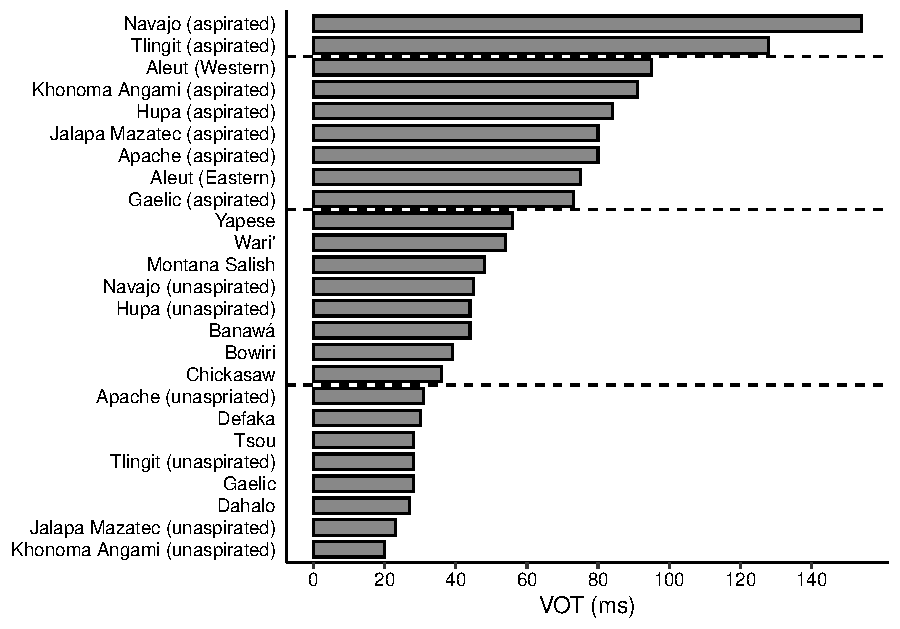
\includegraphics[width=\linewidth]{figures/ch2/real_vot.pdf}
\caption[Mean VOT values for velar stops from eighteen languages in the study of \cite{ChoLadefoged1999}]{Mean VOT values for velar stops from eighteen languages in the study of \cite{ChoLadefoged1999}. Dashed lines indicate the category boundaries assumed by the authors.}
\label{fig:cho_ladefoged_1999}
\end{figure}

To illustrate this point, if language drew on a fixed set of phonetic categories, the picture obtained by \cite{ChoLadefoged1999} should look more like the simulated data shown in Figure \ref{fig:simulated_vot}. Compared to this figure, the original picture resembles a continuous increase of VOT lacking clear jumps between the putative categories. Although this remains pure speculation, it is in line with \citet[42]{Ladd2014} who concludes that ``any apparent discontinuities in the gradual increase from one end of the VOT scale to the other would disappear" when more data were added to the picture of Cho and Ladefoged.

\begin{figure}
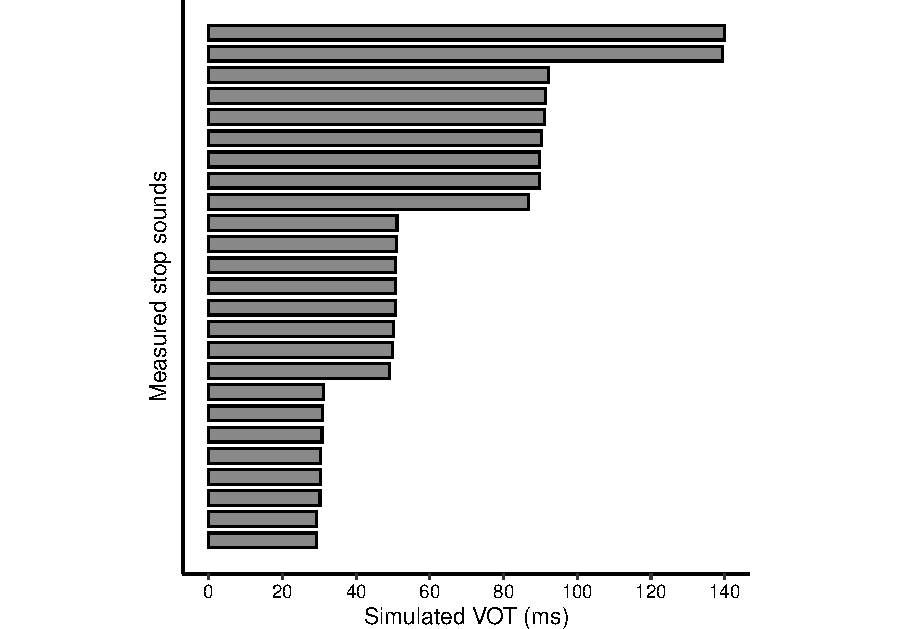
\includegraphics[width=\linewidth]{figures/ch2/simulated_vot.pdf}
\caption{Simulated VOT values under the assumption of a universal set of phonetic categories.}
\label{fig:simulated_vot}
\end{figure}

The idea of a universal set of phonetic categories is an integral part of a \emph{modular} view of phonetics and phonology. As mentioned above, the phoneme was seen as a psychological unit and supposed a division of the abstract representation in the mind and the physical realisation. In this way, phonetics and phonology are conceptualised as two modules from a cognitive perspective. More recent views that dispense with the phoneme and instead assume other representations like feature bundles adhere to a perspective in which modularity plays an important role.

In this perspective of modularity, phonological entities are stored and processed in one module and then passed on to a separate phonetic module to prepare and realise the implementation. Thus, phonetics and phonology are not only separated as scientific disciplines but also viewed as two disparate cognitive domains. Importantly, the separation into clear-cut cognitive modules necessitates translations from symbolic representations to continuous properties \citep{Ohala1990,GafosBenus2006} at the \emph{interface between phonetics and phonology} \citep{Keating1988} -- a term extensively discussed in the last decades. Because the domains are encapsulated and administer their own representations and carry out their own computations before passing the result to the next module, the receiving module cannot access the history of steps that lead to this particular representation. As  \citet[102]{Pierrehumbert2002} notes, the mainstream view of phonetics, phonology and their interface is architectured as a \emph{feed-forward} system ``because no arrows go backwards, from articulatory plans to phonological encoding".

\section{Gradience}
In the above outlined perspectives of phonology, its representations must only entail those features of sounds that cause differences in terms of lexical meaning. The continuous aspects of speech live only on the level of phonetic representations and come into being mainly as a consequence of universal characteristics of articulation, acoustics and audition. The phonological representations are discrete symbols that can be changed by applying discrete rules. An example for such a rule is the assimilation rule given in \ref{eq:assimilation_rule} as taken from \citet[262]{Nolan1992}. In this example, a unit characterised by the features [+coronal], [+anterior], and [$-$continuant] inherits the values of these particular features from the following unit. If this rule is applied to the sequence /leɪt kɔːlz/ (\emph{late calls}), the result would be [leɪk kɔːlz]. 

\begin{equation}
\begin{bmatrix} 
+\text{coronal}\\
+\text{anterior}\\
-\text{continuant}
\end{bmatrix} 
\rightarrow
\begin{bmatrix} 
\alpha \,\, \text{coronal}\\
\beta \,\, \text{anterior}\\
\gamma \,\, \text{continuant}
\end{bmatrix}
/\underline{\hspace{1cm}}
\begin{bmatrix} 
\alpha \,\, \text{coronal}\\
\beta \,\, \text{anterior}\\
\gamma \,\, \text{continuant}
\end{bmatrix}
\label{eq:assimilation_rule}
\end{equation}

Note how the /t/ turned into a [k] – one discrete entity was transformed into another discrete entity. \citet{Nolan1992} demonstrates, using electropalatography (EPG), that the process of assimilation is in fact a gradient process. This means that there are instances of /t/ for which it is possible to find the residual of an alveolar closure during the phase of the plosive. In some instances, there is no complete alveolar closure, but the tongue still has contact to the front parts of the gum. In other instances, the assimilation is complete and the contact is only velar. In these instances, the contacts are comparable to a /k k/ sequence as in /meɪk kɔːlz/ (\emph{make calls}). In addition to showing that assimilation is a gradient process rather than a discrete process in speech production, Nolan also provides evidence that listeners are able to use this gradient information in perception.

A framework that is able to capture gradient phenomena like this is \emph{Articulatory phonology} \citep{BrowmanGoldstein1986,BrowmanGoldstein1992}. In Articulatory phonology, speech sounds are not represented as symbolic units. Instead, the primitives of phonology are gestures. Patterns of speech sounds come into existence through the orchestration of multiple gestures in \emph{gestural scores}. These scores build higher forms, like syllables and words. Crucially, a gesture is viewed as a continuous dynamical system. This makes it possible to describe fine-grained differences in the spatial and temporal manifestations. Assimilation of a /t/ towards a /k/, like in the study of Nolan discussed above, is ascribed to an overlap of the tongue tip gesture for the alveolar closure and the tongue back gesture for the velar closure. The overlap of the two gestures can take any value on a continuous scale from no overlap to complete overlap. In this view, the timing relation of the two gestures is gradient and so is the phenomenon of assimilation. To illustrate how assimilation is modelled in Articulatory phonology, Figure \ref{fig:score_late_calls} shows gestural scores for two instances of \emph{late calls}.\footnote{The scores shown here might not provide a full detailed account of the gestural activations for this phrase, as for example the /l/ in English in word-medial positions is often described as ``dark". Therefore, /l/ in English may be better described by a tongue tip and a tongue back gesture that vary in the degree of overlap.}

A gestural score is a tabular visualisation of the gestural activations during the production of a word or phrase. The vertical axis shows the \emph{tract variables} that correspond to the recruitment of the articulators. In the cases shown here, tongue tip (TT), tongue body (TB) and glottis (GLO) are displayed. There are many more tract variables available in the Articulatory phonology modelling approach, for an overview see \cite{BrowmanGoldstein1992} and \cite{Mücke2018}, as well as the next chapter. The horizontal axis of the gestural score displays \emph{time} such that if an interval starts to the right of another interval, it is said to start later. The boxes give the description of the \emph{location} and \emph{degree of constriction} in a tract variable. The constriction locations used in the score in Figure \ref{fig:score_late_calls} are alveolar (alv), palatal, velar and uvular. The constriction degrees used in the scores comprise two types of closure: clo, denoting a full closure, and clo*, denoting a partial closure with a lateral opening. In addition, critical (crit) stands for a very narrow constriction resulting in friction noise. Finally, the degrees of constriction for the vowels used here are narrow and mid. For the glottis, wide simply indicates that the glottis is open for voiceless, it is closed for voiced otherwise.

\begin{figure}[b]
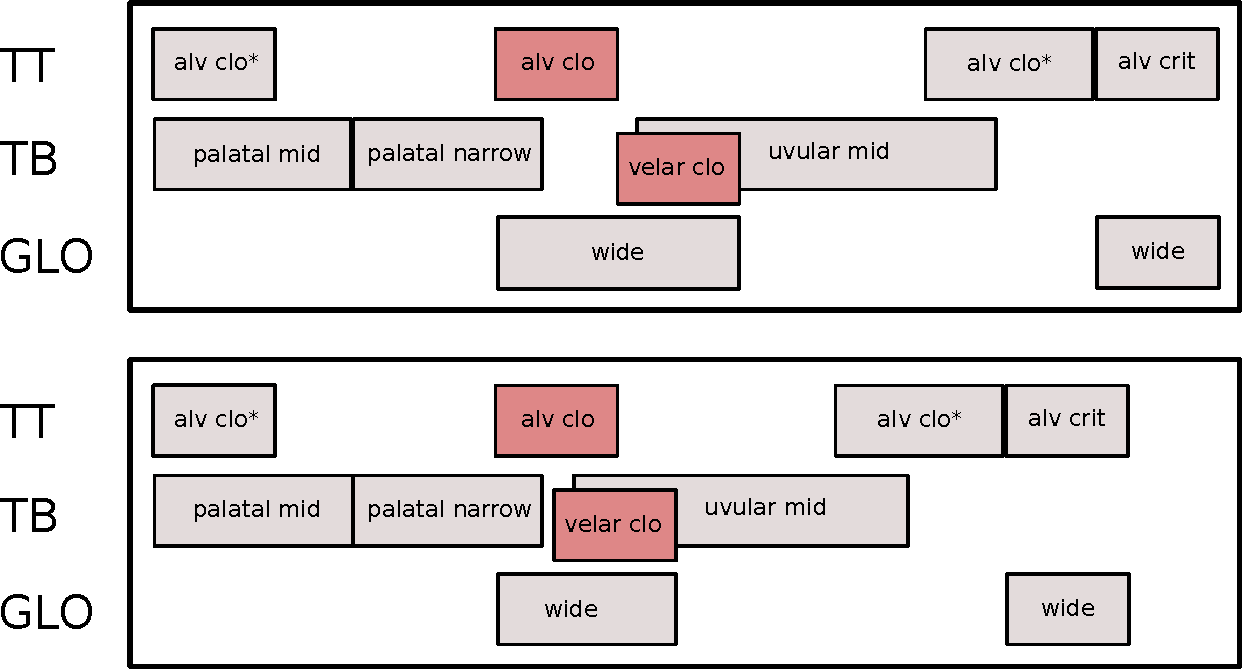
\includegraphics[width=\linewidth]{figures/ch2/late_calls.pdf}
\caption[Gestural scores of the utterance \emph{late calls}.]{Gestural scores of the utterance \emph{late calls} with no overlap of the two stop sounds (top) and high degree of overlap of the two stop sounds (bottom).}
\label{fig:score_late_calls}
\end{figure}

The example shows how the gestural organisation of Articulatory phonology models the gradience of a process like assimilation as continuous variation in the overlap of gestures. In the score at the top of Figure \ref{fig:score_late_calls}, there is no overlap between the alveolar closure gesture of the tongue tip (alv clo in the TT row) and the velar closure gesture of the tongue body (velar clo in the TB row). This score corresponds to a rather careful, clear rendition of \emph{late calls} that results in a clear differentiation of the velar and the alveolar stop. In the score at the bottom of the figure, the two gestures overlap to a large degree. In the acoustic signal corresponding to this score, the two stop sounds would not be differentiated well and hence assimilation would be recorded in a symbolic transcription. However, there is no manipulation or transformation of the set of phonological units involved here as in the rule of \ref{eq:assimilation_rule} where one symbolic representation was replaced by another. The framework models the process as a gradient change in a continuous phonological representation. Although the boxes and labels (e.g. mid vs. wide) in the gestural score make the modelling approach appear discrete, one has to bear in mind that the boxes and labels are just ``shortcuts". A gesture is defined as a continuous dynamical system \citep{BrowmanGoldstein1992,Hawkins1992}, constriction place and degree can vary continuously in this system. In consequence, a label like ``mid" stands for a scalar value on a continuous scale of constriction degree and not for a discrete symbol from a finite set.

The case of assimilation as described above is an example of \emph{gradience} in speech -- a concept that has gained growing attention in recent research in phonetics and phonology \citep{Cohn2006}. Since it is used to denote similar but different phenomena, the term gradience has to be differentiated here. \cite{Ladd2014} referring to \cite{Bolinger1961} distinguishes \emph{physical} from \emph{statistical} gradience. While physical gradience refers to detailed variation on a continuous scale, statistical gradience denotes variation in the statistical patterns of occurrence of an event that can be described as categorical. This differentiation will be referred to in the further course of this work. However, to avoid confusion with other uses of gradience, I will adopt a different terminology. Many scholars use the word gradience to exclusively describe what Ladd calls physical gradience, not statistical gradience. Hence, I will adopt the term \emph{variation} instead. Because statistical gradience or variation refers to the occurrence of categorical events or entities, the term \emph{categorical variation} will be used. Further, I will use the term \emph{continuous variation} to refer to what \cite{Ladd2014} calls physical gradience. 

Various theoretical frameworks have dealt with the development of an accurate description of variation. Articulatory phonology, as demonstrated above, provides a means to account for continuous variation as in the case of assimilation. Of course, using the ends of the continuum, it is also suited to describe categorical variation (e.g. no overlap vs. complete overlap). But most theories have focussed mainly on a categorical description of variable patterns in speech sounds. In turning to patterns of language usage, scholars in the variationist tradition of sociolinguistics decades ago acknowledged that multiple forms of a word may coexist. As a consequence, the rule-based framework endorsed by generative phonology was extended to entail variable rules \citep{Labov1969,CedergrenSankoff1974,Anttila2007}. A variable rule is applied optionally with a specific quantity that denotes how often the rule will be applied. Such a rule may be written in the form X $\rightarrow$ (Y) / A\_B with the parentheses indicating that the outcome of the rule is not generated in all cases (``X optionally turns to Y in the context between A and B").

Other modelling approaches that are able to describe patterns of categorical variation are stochastic extensions of \emph{Optimality Theory} (\citealp{PrinceSmolensky2004}; henceforth: OT). OT is a theoretical framework that works with symbolic representations but without rules. Instead, it uses ranked \emph{constraints} to evaluate the ``winner" from a set of possible \emph{output form} candidates for a given \emph{input form} \citep{Gussenhoven2004}. The winning output form is said to optimally satisfy the constraints and is delivered to phonetic implementation. The tableau in \ref{eq:ot_example} gives a simplified example for computation of the plural form of the English word \emph{kiss} from \cite{GussenhovenJacobs2011}. It uses the constraint \textsc{*SibSib} that is violated if the word contains two adjacent sibilants, the constraint \textsc{Dep-IO} that is violated if a segment not present in the input form is inserted, and the constraint *$\alpha$\textsc{voice}-$\alpha$\textsc{voice} that is violated if two adjacent sibilants do not share the same quality for the voicing feature (e.g. voiceless may not be followed by voiced). The constraints are ranked from left to right: \textsc{*SibSib} outranks \textsc{Dep-IO}, \textsc{Dep-IO} outranks *$\alpha$\textsc{voice}-$\alpha$\textsc{voice}. The symbol * denotes one violation of a constraint for the candidate in that row. The symbol ! indicates whether this violation is ``fatal" which means that this violation leads to the ``defeat" of this candidate. In the example in \ref{eq:ot_example}, candidate b is the only candidate that does not violate the constraint of the highest rank, \textsc{*SibSib}, and thus is the optimal form, marked with the symbol ☞. Of the two violations for candidate a, the violation of \textsc{*SibSib} is fatal because it already renders it a loser of the competition regardless of its violation of *$\alpha$\textsc{voice}-$\alpha$\textsc{voice}.
	
\begin{equation}
\begin{tabular}{|r|c|c|c|}
\hline
/kɪsz/ & \textsc{*SibSib} & \textsc{Dep-IO} & *$\alpha$\textsc{voice}-$\alpha$\textsc{voice} \\
\hline
a. kɪsz &  *! &  & *\\
\hline
☞  b. kɪsɪz &  & * & \\
\hline
c. kɪzz & *! & & \\
\hline
d.  kɪss & *! & & \\
\hline
\end{tabular}
\label{eq:ot_example}
\end{equation}

\largerpage
As can be seen in this simple example, a basic OT approach determines a single optimal form – and the same optimal form will be evaluated by the grammar every time unless the constraint ranking is changed. To implement categorical variation, a probabilistic mapping of input and output form, this account has to be extended. To illustrate the process, one case that will be treated more in-depth here is the probabilistic choice of suffixes in Hungarian \emph{vowel harmony} \citep{HayesLonde2006}. Vowel harmony has been described as a phenomenon in which the vowels within a word agree with regard to some phonetic property, like the place feature [±back] \citep{GafosBenus2006}. In Hungarian, for many stems, the quality  [±back] of the stem vowel determines the choice of the suffix such that the suffix agrees with the stem in its [±back] property. For example, the stem \emph{ablak} /ɔblɔk/ (`window') in which the last vowel is [+back] takes the suffix \emph{nak} /nɔk/ with a back vowel while the stem \emph{üst} /yʃt/ (`cauldron') with a front vowel takes the suffix \emph{nek} /nɛk/ with a front vowel \citep[62]{HayesLonde2006}. In addition, front unrounded vowels function as \emph{transparent or neutral vowels} \citep{HayesLonde2006}. These vowels can occur between the vowel triggering the vowel harmony and the target of the vowel harmony, e.g. the suffix vowels in the examples above, but do not affect the process of vowel harmony – even if their quality of the feature [±back] is opposing to the triggering vowel. For instance, the stem \emph{kávé} /kaːveː/ (`coffee') takes the suffix \emph{nak} /nɔk/ – the back vowel of the stem determines the vowel of the suffix regardless of the intervening unrounded front vowel. 

\largerpage
Interestingly, stems with a back vowel and one or two transparent vowels have been observed to be able to take back and front suffixes, with statistical preferences for one or the other. For instance, \citet{HayesLonde2006} observed that the stem /aːɲiveːl/ occurs with the suffix \emph{nek} /nɛk/ in 83.6\% of cases and with the suffix \emph{nak} /nɔk/ in the remaining 16.4\% of cases. The authors use stochastic OT \citep{Boersma1997,BoersmaHayes2001} to model this probabilistic suffix alternation. To give a full account is beyond the scope of this chapter. The following description is restricted to a short overview to exemplify how stochastic OT can account for categorical variation. The constraint rankings are not strict in this approach, rather the constraints are assigned ranking strength probabilities. The tableau in \ref{eq:stochastic_ot_table} uses three constraints: \textsc{Local[NN]} which is violated when a stem with two neutral vowels is followed by a back vowel, \textsc{Local}[e:] which is violated when the closest vowel following [e:] is a [+back] vowel, and \textsc{Distal[B]} which is violated when a [+back] vowel is followed by a [$-$back] vowel somewhere in the word.\footnote{This is not the complete set of constraints used by \citet{HayesLonde2006} to model the data, it represents a minimal example to illustrate the point of probabilistic constraint rankings.} The fact that they are not ranked strictly (or statically) as in the previous example is expressed by the dashed separation lines between the columns. The ranking strengths of the constraints are given by the probability density functions shown in Figure \ref{fig:probs_stoch_ot}. \textsc{Local[NN]} has a mean ranking strength of 101.802, \textsc{Local}[e:] has a mean ranking strength of 100.894, \textsc{Distal[B]} has a mean ranking strength 100.000. The standard deviation is 2 in all cases. From these ranking strength distributions, the probability for a given output form can be calculated. Candidate a in tableau \ref{eq:stochastic_ot_table} from \citet[81]{HayesLonde2006} violates \textsc{Distal[B]} three times, candidate b violates the other two constraints but \textsc{Distal[B]} only twice. For candidate b to win, the constraint \textsc{Distal[B]} has to be outranked by both \textsc{Local[NN]} and \textsc{Local}[e:]. The question is: If one ranking strength sample is taken from each of the three distributions presented in Figure \ref{fig:probs_stoch_ot}, how often will the two samples for \textsc{Local[NN]} and \textsc{Local}[e:] both be smaller than that for \textsc{Distal[B]}? The answer is: In 16.4\% of all cases. In all other cases, candidate a will win. The probabilities are given in the first column, to the left of the candidates.

\begin{equation}
\begin{tabular}{|r|c:c:c|}
\hline
/aːɲiveːl-nAk/ 		& 	\textsc{Local[NN]} & 	\textsc{Local}[e:] &		\textsc{Distal[B]} \\
\hline
0.836 ☞ a. aːɲiveːl-nɛk & 			         & 			       &		***(!) \\
\hline
0.164 ☞ b. aːɲiveːl-nɔk 	&         *(!)		         &	*(!)                       &       	 **\\\hline
\end{tabular}
\label{eq:stochastic_ot_table}
\end{equation}

\begin{figure}
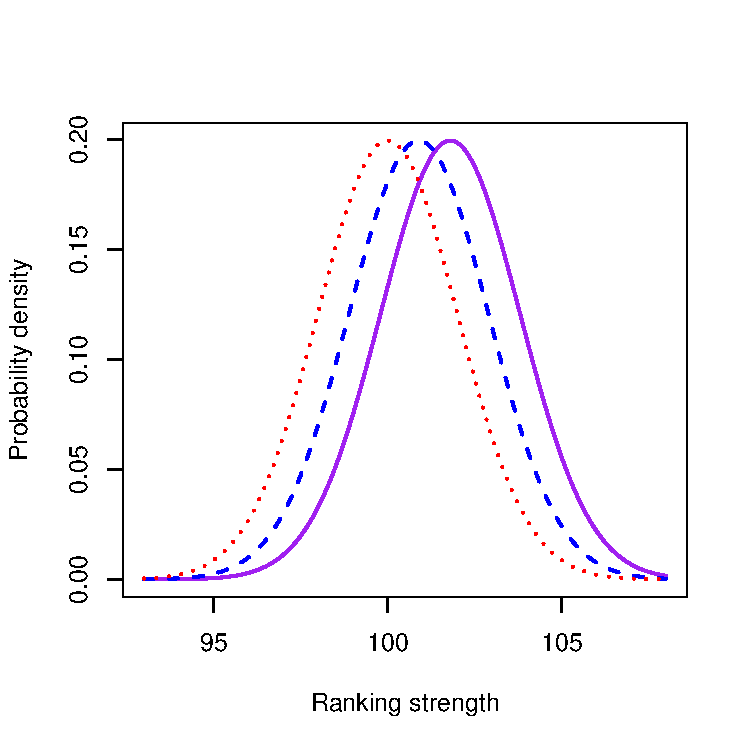
\includegraphics[width=9cm]{figures/ch2/stochastic_ot.pdf}
\caption[Ranking strength probabilities for the constraints of \citet{HayesLonde2006}.]{Ranking strength probabilities for the constraints based on footnote 15 of \citet{HayesLonde2006}. \textsc{Local[NN]} (purple, solid line), \textsc{Local}[e:] (blue, dashed line), \textsc{Distal[B]} (red, dotted line).}
\label{fig:probs_stoch_ot}

\end{figure}

As becomes clear from this example, stochastic OT is able to cope with statistically gradient patterns, or categorical variation, i.e. the statistical preference for one or another category. Continuous variation is not captured by this framework. In the next chapter, a dynamical systems approach to the problem of the probabilistic suffix choice in Hungarian will be outlined that focusses on continuous sub-symbolic variation \citep{GafosBenus2006}. This model builds on articulatory details and shows how continuous variation may contribute to categorical variation. 

As outlined in the introduction to this book (Chapter \ref{chapter_intro}), it is one of the aims of the present work to show that categorical and continuous variation often go hand in hand. This view is in line with \citet[88]{Ladd2014} who notes that ``[i]n many situations, of course, the two types of variation are likely to interact and reinforce one another." Motivated by the fact that categorical and continuous phenomena in speech often show a high degree of parallelism, \citet{Flemming2001} presents a model rooted in OT that combines continuous and categorical aspects and intends to reconcile phonetic and phonological representations in a formal approach. The main idea revolves around a trade-off of constraints rather than a categorical ranking of constraints. This trade-off can be determined by expressing the violation of each constraint as a scalar quantity. As a result, each possible candidate of the optimalisation process acquires a cost and the candidate with the lowest cost is selected as the optimal form. This approach will be outlined here in more detail using the example of assimilation of a back vowel to a coronal consonant.

It has been observed that in some languages the contrast between front and back rounded vowels is neutralised in the position between coronal consonants. For example, in Cantonese Chinese the two  forms /kʰyt/ (`decide') and /kʰut/ (`bracket') exist, as well as /tʰyt/ (`to take off'). There is, however, no form */tʰut/ \citep{Flemming2001}. This phenomenon has been described as a case of categorical assimilation, i.e. as the outcome of a phonological computation in which the  [+back] specification of the vowel is changed to [+front]. In other languages, a parallel process, the co-articulatory fronting of back vowels in the context of coronal consonants has been described as purely phonetic (and as such continuous). In English, for example, /u/ is produced more fronted in \emph{toot} /tut/ compared to \emph{coo} /ku/.

The modelling idea of \citet{Flemming2001} involves the formulation of the following constraints based on a quantification of the second formant (F2) of both the consonants and the vowel. The constraint \textsc{Ident(C)} requires the target F2 of a consonant to be maintained. Its violation cost is the weighted squared difference between the realised F2 of the consonant and the target F2 of the consonant: $weight_c \cdot (F2(C) - L)^2$, where $F2(C)$ is the realised F2 of the consonant and $L$ is the target F2 of the consonant.

The constraint \textsc{MinimiseEffort} requires that the speaker reduces articulatory effort. It tries to keep changes in F2 from C to V as small as possible. Its violation cost is the squared difference between the realised F2 of the consonant and the realised F2 of the vowel: $weight_e \cdot (F2(C) - F2(V))^2$, where $F2(C)$ is the realised F2 of the consonant and $F2(V)$ is the realised F2 of the vowel.

The constraint \textsc{MinDist  = Δ} requires that the distance between the F2 of the vowel /u/ and its nearest neighbour /y/ is above a certain threshold. Its violation cost is the weighted difference between the distance of /u/ and /y/ in terms of F2 and the threshold: $weight_v \cdot (|F2(y) - F2(u)| - \Delta)^2$, where $F2(y)$ is the F2 of the vowel /y/, $F2(u)$ is the F2 of the vowel /u/, and Δ is the minimum distance between the two, the threshold. This constraint only applies if the contrast is maintained. Its violation cost is not calculated if the contrast is neutralised, i.e. the assimilation is categorical.

In addition, the model uses the quantity \textsc{MaximiseContrast}. This value represents the benefit of preserving a contrast. While the other three constraints acquire positive costs as they are violated, \textsc{MaximiseContrast} is subtracted as a negative cost.

The candidates of the optimisation process are inventories of contrasting syllables. First, the total violation cost for a candidate is calculated as the sum of all single weighted violation costs for the constraints. Second, the benefit of maintaining the contrast, \textsc{MaximiseContrast}, is subtracted. After these steps, the inventory with the lowest cost is selected as optimal. Thus, if the benefit of maintaining the contrast is exceeded by the costs obtained by the distinctiveness and effort constraints (\textsc{Ident(C)}, \textsc{MinDist = Δ}, and \textsc{MinimiseEffort}) in the realisation of /tut/, it is optimal to neutralise the contrast between /u/ and /y/. The consequence is \emph{categorical assimilation}. On the contrary, if the combined costs for the violation of the constraints \textsc{Ident(C)}, \textsc{MinDist = Δ}, and \textsc{MinimiseEffort} do not exceed \textsc{MaximiseContrast}, neutralisation in the form of categorical assimilation is not optimal. However, as a trade-off between \textsc{Ident(C)} and \textsc{MinimiseEffort}, \emph{co-articulatory assimilation} with varying degrees follows. In this model, the difference between languages can be modelled by using the same sets of constraints and modulating the value for \textsc{MaximiseContrast} as well as the weights for the violation costs of the constraints as scalar values. Depending on how the weights are set, the costs for distinctiveness and effort might exceed the benefit of maintaining a contrast or not \citep{Flemming2001}.

Similar to Articulatory phonology, Flemming's approach models degrees of assimilation in the same formal system and does not distinguish between categorical, phonological and continuous, phonetic processes. In Articulatory phonology, assimilation is a fundamentally continuous process as the organisation of gestural activation varies on the continuous dimension of time -- affecting the temporal and spatial properties of the phonetic outcome. Categorical behaviour can be found at the ends of the continuum. In Flemming's model, the trade-off between the benefit of contrast preservation and the costs connected to effort and distinctiveness of sound pattern explains the outcome as categorical or continuous assimilation. In both modelling frameworks, categorical variation on the ``macro-level" is seen as the result of the interaction of variation on continuous dimensions on the ``micro-level".

\section{Tiny differences, rich memory}
Another famous example that poses a problem for the modular view of phonetics and phonology is the phenomenon known as \emph{incomplete neutralisation}. It describes the finding that the neutralisation of the voicing contrast of syllable-final obstruents present in some languages as the result of \emph{final devoicing} is indeed incomplete. Final devoicing or \emph{Auslautverhärtung} is a classic textbook example showing that voiced obstruents at the end of syllables turn into voiceless obstruents in German. Thus, the contrast between voiced and voiceless is said to be \emph{neutralised} in this context. Similar phenomena have been observed in other languages as well \citep{Bloomfield1933}. In a modular, symbolic account of the case, the voiced obstruent is transformed into a voiceless obstruent at the end of syllables by virtue of a phonological rule like the one given in \ref{eq:final-devoicing} (where \$ stands for the end of a syllable). This rule is suited to turn a structure like /ʁad/ into [ʁatʰ] and thus makes the difference between the phonetic outputs of the words \emph{Rad} (`wheel') and \emph{Rat} (`advice') disappear completely.

\begin{equation}
\text{[+voiced]} 
\rightarrow 
\text{[$-$voiced]}
/\underline{\hspace{1cm}}\$
\label{eq:final-devoicing}
\end{equation}

Contrary to the prediction of this rule, a considerable number of studies found that the acoustic signals of words like \emph{Rat} and \emph{Rad} are different \citep{DinnsenGarciaZamor1971, PortODell1985, CharlesLuce1985, PortCrawford1989, ErnestusBaayen2006, Roettgeretal2014}. In general, the voicing contrast can be encoded by different phonetic cues like glottal pulsing in the closure of the stop, closure duration, voice onset time, but also duration of the preceding vowel \citep{Lisker1986}. Studies on the incompleteness of the voicing contrast demonstrated that the differences between the acoustic signals regarding these parameters go in the direction of a voicing contrast in inter-vocalic position as in \emph{Räder} vs. \emph{Räte}, although the differences are much smaller. Recently, \cite{RoettgerBaerHenney2019} added convincing empirical evidence for the robustness of the incompleteness of German final devoicing using a large, diverse data set.

An approach based on discrete symbolic representations and rules, like the one outlined in \ref{eq:final-devoicing}, is clearly not able to account for the continuous, subtle variation reported by the studies above. The question arises how the difference between the two obstruents can be best captured in a model of phonetics and phonology. An early proposal by \cite{PortODell1985} is to employ \emph{phonetic implementation rules}. While phonetic implementation rules were already implicitly assumed by earlier models \citep[like][]{ChomskyHalle1968, JacobsonFantHalle1952}, they were not considered linguistic in a strict sense, i.e. not part of langue. \cite{PortODell1985} extend the classic model of separated phonetics and phonology by considering language-specific phonetic implementation rules that belong to the speaker's knowledge of the language. To account for the incompleteness of final devoicing in German, the authors use a rule that phonetically implements the syllable. It is the duty of this rule to devoice a voiced obstruent at the end of syllables. Thus, the voiced obstruent retains its phonological specification [+voiced] during the stage of phonological derivation. Only later, at the stage of phonetic implementation, a gesture is activated that resembles the one found with sounds that possess the phonological quality [$-$voiced]. 

While the inclusion of a phonetic rule that is in fact part of the language ``makes the relationship between phonetics and phonology closer by permitting the phonetic implementation system to directly execute the macrostructures in the phonology” \citep[468--469]{PortODell1985}, it strictly adheres to the modular view of phonetics and phonology. In fact, it emphasises the separation between the two modules despite making them more similar. In a footnote, \cite{PortODell1985} entertain the interesting idea that \emph{rules} might not be the right devices in general to account for the cognitive underpinnings of language and speech. In the next chapter (Chapter \ref{chapter_ds}), a dynamical model for the subtle differences observed in the syllable-final obstruents in German is introduced \citep{Gafos2006, GafosBenus2006}. This model does not assume rules or a separation of categorical and continuous aspects. As will become clear in this chapter, despite using a continuous formalism, the model is nevertheless able to explain the categorical nature of the [±voiced] feature.

Other accounts have modelled the phenomenon as an artefact of lexical co-activation, also known as \emph{phonetic paradigm uniformity}, without the need for the invention of a new kind of rules \citep[e.g.][]{ErnestusBaayen2006, GoldrickFolkRapp2010, KleberJohnHarrington2010, WinterRoettger2011, Roettgeretal2014, SeyfarthKlokGarellek2019}. The basic idea behind these approaches is that the mental lexicon stores a collection of rich auditory forms of words, like \emph{Rad}, \emph{Räder}, and \emph{Rades}, rather than abstract representations and rules to produce derived forms. During the activation of a word like \emph{Rad}, close lexical neighbours like \emph{Räder} and \emph{Rades} are co-activated. These co-activated forms enhance the probability that the final obstruent of \emph{Rad} is realised with phonetic characteristics slightly pushed in the direction of a voiced obstruent \citep{ErnestusBaayen2006, Roettgeretal2014}. 

These approaches are rooted in a framework known as \emph{exemplar theory}. Exemplar theory, originally proposed in psychology for the classification of multi-dimensional stimuli more generally \citep{Nosofsky1986, Hintzman1986}, has gained a lot of attention in phonetics and phonology. It postulates detailed, episodic memory of acoustic traces of words as the basis of speech production and perception \citep[among others]{Goldinger1996, Johnson1997, Pierrehumbert2001, Bybee2001, Pierrehumbert2016}. Exemplar theory is thus fundamentally different from rule-based or constraint-based theories of phonology which, as outlined above, assume abstract units to achieve ``maximally simple, redundancy-free representations" \citep[213]{GahlYu2006}. Exemplar theory postulates that the detailed experiences of language use shape the cognitive representation of speech sounds through memorisation of the particular signal (or at least parts of it). Every time a speaker hears a word -- be it spoken by another person or herself -- a new acoustic trace called \emph{exemplar} is stored in her memory near the location of the existing exemplars. During the perception and the production of speech sounds, clouds of stored exemplars are activated. In the case of categorisation, the incoming stimulus is compared against the rich inventory of exemplars. The stimulus will be categorised as belonging to the group of stored exemplars that are most similar. In the case of production, the stored clouds of exemplars serve as production targets. In both perception and production, newer exemplars have more influence since memory traces fade away over time \citep{Schweitzer2012}.

Exemplar models are able to account for experimental findings demonstrating the importance of fine-grained phonetic detail in both perception and production \citep{Pierrehumbert2016}. For example, \cite{Wright1979} as well as \cite{Jurafskyetal2002} showed that more frequent words are produced faster and more reduced compared to less frequent words. This finding also applies to words that are more predictable from the context \citep{Seyfarth2014, AylettTurk2004, Halletal2018}. From an exemplar-based perspective, articulatory effort can be seen in relation to the likelihood of activation. A lexical item with a large cloud of exemplars is activated more easily than a lexical item with a smaller cloud. As outlined above, each time a word is perceived, its acoustic trace is added to the existing exemplars. Hence, less articulatory effort is needed for the transmission of words that are heard very frequently since their exemplar clouds generally accumulate more traces. 

In addition to frequency, lexical access can also be facilitated by many other factors, like indexical information about the speaker producing the word: \cite{WalkerHay2011} showed that listeners were faster and more accurate in lexical decision for words that are more frequently heard in real life said by older speakers, like \emph{typist}, when these words are produced by an older voice in the experiment. Vice versa, words that are more frequently heard in real life from younger speakers, like \emph{checkout}, were more easily processed in the experiment when produced by a younger voice.

Exemplar theory emphasises the importance of phonetic detail for our understanding of speech and offers a completely different view on the relation between phonetics and phonology. While abstractionist frameworks like the rule-based or constraint-based models presented in this chapter view phonology as a reduced, abstract structure that is efficient in terms of memory consumption, exemplar theory posits that the speaker stores and uses large pools of real, experienced ``data". While abstractionist models operate on segment-sized units that in some sense adhere to the phonemic principle, exemplar theory uses larger chunks like words. Scholars in the abstractionist tradition have often highlighted that segment-based approaches are good at explaining the regularities in sound change throughout the whole phonological system, like \emph{chain shifts} described by Grimm's law \citep{Guy2014}. Exemplar theorists on their part have argued that sound changes may not necessarily be regular. While Middle English long /o/ in today's English turned into /u/ in words like \emph{root} and \emph{food}, it also developed into /ʊ/ in words like \emph{good} and \emph{book} or schwa as in \emph{flood} \citep{Guy2014}. However, pure exemplar approaches have difficulties dealing with regularities in sound change – even if these regularities might not complete \citep{Pierrehumbert2016}. Further critique towards purely ``data-driven" exemplar models includes evidence that in addition to \emph{token frequency} (accumulated traces of perceived words), \emph{type frequency} of a lexical unit plays a role for the productivity of this pattern \citep{HayPierrehumbertBeckman2004}. 

As a consequence, exemplar-based approaches have been extended to \emph{hybrid models} which argue that abstract phonological representations also play a role. One of these models is delivered by \cite{Pierrehumbert2002} positing that abstract generalisations and exemplar clouds can be associated with phonological units like phonemes, sequences of phonemes, or words \citep[see also][]{GermanCarlsonPierrehumbert2013}. The model makes a distinction between production and perception. In production, phonological units play a major role but exemplars bias the production goals of the abstract units. On the contrary, in perception, exemplars play the leading role. The related \emph{Polysp} model \citep{HawkinsSmith2001, Hawkins2003} emphasises that identification of meaning in communication ``takes place probabilistically, using all possible available information in parallel to flesh out linguistic structure at all levels" \citep[391]{Hawkins2003}. Following this model, a listener might analyse a given acoustic signal into abstract linguistic units and match the signal with exemplars \citep{Ernestus2011}. Notably, in \emph{Polysp}, exemplars can include non-acoustic memory like visual information. \citet[8]{Sumneretal2014} endorse a similar view stating that ``[l]isteners simultaneously extract linguistic and social information from speech". While hybrid approaches offer promising explanations and testable predictions, \cite{Ernestus2011} notes that a full computational implementation of these models is still in progress.

\section{Summary}
In this chapter, the relation of phonetics and phonology was explored. It was outlined that the 20th century, with the rise of the phonemic principle, introduced a rather sharp separation between continuous, physical phonetics and categorical, symbolic phonology -- a distinction that was weaved into the fundamentals of linguistics. Even models in the tradition of \citet{ChomskyHalle1968} that dispense with the concept of the phoneme in a strict sense maintain the split as an important assumption. The chapter reviewed some of the problems which challenge a clear-cut separation and highlighted that many scholars nowadays assign a significant role to fine phonetic detail in cognitive representations of sound patterns as well as storage in memory. In this context, it becomes increasingly important to investigate how theoretical approaches are able to deal with continuous and categorical variation in sound patterns and linguistic structure. Models rooted in the framework of dynamical systems offer promising solutions for reconciling the continuous and categorical aspects in one formal language. Since the focus of this book is on modelling approaches within this framework and what they have to offer for an understanding of the relation of categorical and continuous aspects of speech, the next chapter introduces the foundations of dynamical systems and reviews important applications.

